\documentclass{article}
\usepackage[utf8]{inputenc}
\usepackage{geometry}
\geometry{verbose,tmargin=4cm,bmargin=3cm,lmargin=4cm,rmargin=3cm}
\usepackage{braket}
\usepackage{graphicx}% Include figure files
\usepackage{dcolumn}% Align table columns on decimal point
\usepackage{bm}% bold math
\usepackage{float}
\usepackage{physics}
\usepackage{verbatim}

\title{Listas 1-6- Fisica Moderna 2}
\author{smendoncabruna }
\date{August 2020}

\begin{document}

\maketitle

\section{Questões}
\subsection{Por que, ao discutirmos as figuras 8-1 e 8-4, falamos em pólos magnéticos fictícios?}

Porque, pelo tratamento via mecânica quântica, temos que os valores esperados das componentes perpendiculares do campo magnético criado por um dipolo quântica se comporta da mesma forma que o que pode ser obtido pela abordagem de física clássica.

\subsection{Por que o torque que atua sobre um dipolo magnético num campo magnético faz o dipolo precessionar em torno do campo em vez de alinhá-lo ao campo?}

O momento de dipolo não pode se alinhar ao campo magnético sem que haja dissipação de energia, o que não é o caso, por exemplo, num campo magnético não uniforme.

\subsection{Exatamente por que concluímos que os números quânticos de spin são semi-inteiros?}
Pelo experimento de Stern-Gerlach, vemos que as partículas serão defletidas em dois sentidos, para cima e para baixo em relação ao campo magnético. Segundo as previsões da mecênica quântica de Schrodinger, os valores quantizados do momento de dipolo deveriam ser 2l+1, onde l é um inteiro. Isso é inconsistente com a ideia de haveriam duas projeções possíveis. Esse foi um dos motivos para a concepção de um outro número quântico, o spin, que poderia ter valores fracionários. Em particular, o spin s=1/2 cumpre 2(1/2)+1 =2 possíveis projeções.

\subsection{É justo criticar a mecânica quântica de Schrödinger por não prever o spin do elétron?}
A teoria de Schrodinger não estava errada e nem era contraditória a existência de spin. Muitos resultados que envolvem spin, como a previsão da estrutura fina do átomo de hidrogênio, poderiam ser incluidos na teoria e obteriam resultados suficientemente bons (ver primeiro problema da lista).

\subsection{Explique em termos simples por que um elétron num átomo de hidrogênio está submetido a um campo magnético. Este campo existe em todo e qualquer estado quântico?}
Podemos associar uma corrente à carga em movimento e, pela lei de Ampère,  podemos relacionar com um campo magnético. Não contamos com esse campo quando o estado possui l=0.

\subsection{O que é exatamente a interação spin-órbita? Como ela leva ao desdobramento de estrutura fina observado nas linhas espectrais do átomo de H?}
É a energia de interação entre o spin do elétron e o campo gerado pelo fato do elétron possuir uma carga e estar em movimento. Essa energia entra como um termo extra, com ordem de grandeza bem menor do que a energia total, mas suficiente para explicar a divisão das linhas espectrais.

\subsection{Quando se considera a interação spin-órbita, diz-se às vezes que ml e ms não são mais “bons números quânticos”. Explique por que tal terminologia é apropriada. Quais são os bons números quânticos quando a interação spin-órbita é levada em conta?}

Tendo interação spin-orbita, a conservação se refere ao momento total J = L+S. As projeções Lz e Sz não são mais conservadas, então os números quânticos associados a essas grandezas não são mais relevantes para a caracterização de um estado nesse caso. J e mj.

\subsection{Quais são os bons números quânticos para um átomo de um só elétron num campo magnético externo que, comparado ao campo interno, é muito fraco? E muito forte?}

Num campo muito forte, podemos considerar que tanto L quanto S vão precessionar na direção do campo magnético. Assim, ml e ms voltam a ser bons numeros quânticos.
No caso de campo fraco, vale o argumento da questão anterior.

\subsection{Por que a interação spin-órbita é particularmente sensível à forma do potencial V(r) para pequenos valores de r? Como pode isto ser utilizado para o estudo experimental dos potenciais dos átomos multieletrônicos?}
A energia da interação spin orbita depende da derivada de V(r) com relação a r. Se V(r) é sensivel para valores pequenos, a energia de interação será ainda mais sensível.
No caso de átomos multieletrônicos, o potencial tem uma forma diferente de modo que possa corresponder, de forma aproximada, aos efeitos de blindagem das cargas e da interação entre elétrons.
Uma técnica experimental que possui boa concordância com os resultados para átomos multieletrônicos via método de Hartree é o estudo do espectro de emissão de raios-x. É uma forma de medir a energia de camadas mais internas. O aumento uniforme na energia das camadas internas com o aumento da carga Ze foi confirmado por Moseley.

\section{Problemas}
\subsection{Use o procedimento do exemplo 8.3 (pag 360) para estimar a energia de interação spin-órbita no estado n=2 e l=1 de um átomo muônico, definido no exemplo 4-9.}

\nonumber \begin{align}
    &\Delta E \approx 0.2292 eV \\
    &\frac{E_{ligacao}}{\Delta E} \approx 10^4, 
\end{align}
como esperado.

\subsection{Enumere os possíveis valores de j e mj para os estados onde l=3 e s = 1/2.}

j = 7/2, 5/2.
\[ \]
Para j $ = 7/2$, $m_j$ = 7/2, 5/2, 3/2, 1/2, -1/2, -3/2, -5/2, -7/2.
\[ \]
Para j $ = 5/2$, $m_j$ = 5/2, 3/2, 1/2, -1/2, -3/2, -5/2.


\section{Questões Elaboradas}

\subsection{Para estados atômicos com l = 0, a densidade de probabilidade $|\Psi|^2$é máxima na origem. No entanto, a probabilidade de encontrar o elétron a uma certa distância do núcleo, P(r), vai a zero quando r $\to$ 0. Explique.}
As funções radiais tem forma $r \propto e^{r}r^l$. Para r pequeno, $r \propto r^l$, então a densidade de probabilidade é proporcional a $r^{2l}$. No entanto, a função tende a zero muito rapidamente conforme r aumenta. Assim, para l=0, o máximo de probabilidade se encontra na origem e decresce rapidamente.

\subsection{Porque a direção do momento angular orbital de um elétron é oposta à de seu momento de dipolo magnético?}
Isso se deve ao sinal negativo da carga do elétron - se fosse positivo, seria paralelo e não anti-paralelo.

\subsection{Porque, no experimento de Stern-Gerlach, é usado um campo magnético não homogêneo? }
O campo não homogêneo produz uma componente de força na direção de onde aumentam as linhas de campo, ou seja, espera-se que haja uma mudança na trajetória da particula caso ela seja de alguma forma afetada pelo campo magnético.

\subsection{No experimento de Stern-Gerlach poderiam ser usados íons em vez de átomos neutros?}

A ideia de se usar átomos neutros (em particular, átomos de prata, cuja úlltima camada é s) é evitar a influencia do termo orbital para a deflexão das partículas. Deflexão num átomo neutro implica em alguma outra grandeza influenciada pelo campo magnético: o spin.

\subsection{Porque o Lítio, o Potássio e o Sódio exibem propriedades químicas semelhantes?}
Esses elementos são denominados alkalis. Eles possuem um único elétron fracamente ligado em uma camada s (l=0). Isso faz com que seja fácil de ionizar esses átomos. Portanto, é fácil criar reações químicas com esses elementos.

\subsection{Uma energia de 21 eV é necessária para excitar um elétron de um átomo de He do estado 1s para o 2s. A mesma transição, no íon He+, requer aproximadamente o dobro de energia. Explique.}
A energia é, em primeira aproximação, proporcional a carga do nucleo multiplicada pela carga dos elétrons.
Para o Helio ionizado, temos carga 2e do núcleo e carga e do elétron. Para o Helio neutron, temos 2e do núcleo e 2e dos elétrons.

\subsection{O acoplamento spin-órbita quebra a degenerescência de todos os estados, menos os s. Porque eles são exceção?}
Os estados s correspondem a estados com numero quântico l=0. Isso implica em momento angular orbital L=0 e, portanto, termo de spin órbita nulo.

\section{Problemas}
\subsection{Use o procedimento do exemplo 8.3 (pag 360) para estimar a energia de interação spin-órbita no estado n=2 e l=1 de um átomo muônico, definido no exemplo 4-9.}

\nonumber \begin{align}
    &\Delta E \approx 0.2292 eV \\
    &\frac{E_{ligacao}}{\Delta E} \approx 10^4, 
\end{align}
como esperado.

\subsection{Enumere os possíveis valores de j e mj para os estados onde l=3 e s = 1/2.}

j = 7/2, 5/2.
\[ \]
Para j $ = 7/2$, $m_j$ = 7/2, 5/2, 3/2, 1/2, -1/2, -3/2, -5/2, -7/2.
\[ \]
Para j $ = 5/2$, $m_j$ = 5/2, 3/2, 1/2, -1/2, -3/2, -5/2.

\section{Lista 2: Eisberg e Resnick, Cap. 9, questões:}
\subsection{1 - Por que é difícil distinguir os dois elétrons de um átomo de hélio mas não os dois elétrons pertencentes a átomos de hidrogênio separados? E numa molécula diatômica de hidrogênio?
}
A dificuldade em distinguir partículas do mesmo tipo vem da possibilidade de interferências de suas funções de onda. Isso é mais evidente dentre de um próprio átomo do que de átomos externos.

\subsection{4-Ao trabalhar com sistemas quânticos contendo partículas idênticas, não seria questionável a utilização de índices para as partículas? Se não, explique qual a precaução que deve ser tomada ao usá-los.
}
Manter índices é necessário para a clareza dos cálculos apenas, mas não reflete a física. Precisamos incorporar a indistinguibilidade de outra forma. Essa forma é construindo funções de onda nas quais as grandezas físicas são invariantes à troca de índices.

\subsection{5- O valor de uma autofunção total anti-simétrica mudando quando as coordenadas das partículas são trocadas, como poderá ela ser utilizada para dar uma descrição precisa de um sistema de elétrons?
}
A autofunção total não é um observável. Os observáveis derivados da função de onda permanecem os mesmos, então não há problemas.

\subsection{7- Você acha que o sinal da carga de uma partícula elementar, como um elétron ou próton, é uma propriedade mais fundamental ou menos fundamental do que o "sinal" de sua simetria?
}

A propriedade de indistinguibilidade é crucial para a diferenciacao do tratamento classico e quantico, e suas consequencias valem para particulas com qualquer carga. Especialmente porque, em primeira aproximação, nao estamos considerando interação de Coulomb!

\subsection{8- Os átomos seriam mais afetados por uma inversão dos sinais das cargas de todas suas partículas constituintes ou pela troca de todas as suas simetrias?}

Troca de simetria (de permutação, no caso) implica em fermions virando boson e vice versa. Não seria mais um atomo como conhecemos.

\subsection{9- O que significa exatamente a afirmação de que a variável de spin não é contínua?}
O spin apenas assume valores discretos (não um contínuo de valores).

\subsection{11-Por que seria muito mais difícil resolver uma equação de Schrodinger independente do tempo para um sistema de partículas que interagem do que para um sistema de partículas que se movem independentemente?}

Porque levar a interação entre partículas (via potencial coulombiano) em conta criaria um problema de muitos corpos, que é intratável.

\subsection{12- Descreva as etapas de um ciclo do tratamento autoconstistente de Hartree de um átomo multieletrônico. Por que a estimativa do potencial resultante V(r) obtida no fim do ciclo é mais precisa do que a utilizada no inicio?}

1- Chute inicial da forma do potencial, V(r) - dependencia mais forte com a carga do núcleo com a proximidade do elétron com o mesmo.

2- Usar equação de Schrodinger independente do tempo.

3- Obter o estado fundamental minimizando a energia e considerando a condição fraca do princípio da exclusão de Pauli (um único elétron por estado).

4- Cálcular a densidade de carga de cada estado usando as autofunções. As cargas de Z-1 elétrons são somadas ao núcleo e serão a carga sentida pelo elétron restante.

5- Usar a lei de Gauss para calcular o campo elétrico com esses valores e achar um novo valor V(r)

6- Se o valor inicial do potencial e o valor obtido no passo 5 forem muito discrepantes, recomeçar o processo usando o último V(r) obtido. Eventualmente a diferença será irrelevante e esse será o potencial obtido de forma auto-consistente.

\subsection{13- Por que a dependência angular das autofunções de um átomo multieletrônico é a mesma de um átomo monoeletrônico? Por que a dependência radial é diferente, exceto próximo a origem?}

A dependência angular é devido ao uso de um potencial central para facilitar contas na abordagem de Hartree.

Já a dependência radial, que mesmo para átomos monoeletrônicos já possuia particular sensibilidade de l para r pequeno, agora possui mais uma dependência com l. Temos, agora, que levar em consideração 2 possíveis valores de $m_s$ e (2l+1) possibilidades de $m_l$, o que entra como um fator 2(2l+1) na densidade probabilidade radial.

\subsection{14- Qual é a justificativa para o uso das equações dos átomos monoeletrônicos com um Z efetivo para discutir os átomos multieletrônicos?}
O problema de átomos multieletrônicos, quando se leva em conta a interação elétron-elétron, é um problema de muitos corpos, portanto, muito complicado.

Para contornar isso, é feita uma série de aproximações a partir do átomo monoeletrônico, de forma a acrescentar contribuições de energia cada vez menores e obter um resultado mais próximo da realidade. 

A primeira aproximação é considerar a energia entre um átomo de carga Ze e os elétrons, onde Z é uma carga efetiva - a carga média que o elétron sente, considerando, em grosso modo, a atração entre o núcleo e repulsão de outros elétrons.

\subsection{15- Quais as consequências do fato de que o tamanho de todos os átomos seja aproximadamente os mesmos? Quais as razões para esse fato?}

A razão para isso é que o raio cresce devagar com o numero atômico Z. O raio é aproximadamente o mesmo devido ao fato de que, para as camadas externas, o efeito de blindagem faz com que a força de atração seja semelhante com a sentida por um único elétron em um átomo de hidrogênio.
Com o tamanho (valor de r) sendo semelhantes, a diferença na forma da distribuição de probabilidade dependerá mais fortemente do número quântico l, em espacialme para r pequeno. Isso faz com que o conceito de subcamada seja relevante.

\subsection{18- Por que é particularmente difícil separar mistura de elementos de terras raras por processos químicos?}

Porque, para esses elementos, preenche-se a subcamada 4f, que é fortemente blindada do ambiente graças a camada 6s. Assim, difícil acessar suas propriedades químicas, já que são muito parecidas com as de elementos de subcamada 6s.

\subsection{19- Por que podemos ter certeza de que nao existiria vida se não existissem moléculas?}

As moléculas são necessárias para processos bioquímicos, que formam a vida como conhecemos. Sem o princípio de exclusão de pauli, todos os elétrons estariam na camada de menor energia, não teríamos campo elétrico externo, todos os átomos seriam inertes e não formariam moléculas.

\subsection{20- Qual a propriedade dos raios X que os torna tão útil para ver estruturas internas, normalmente invisíveis?}

Com raios X, que são ondas eletromagnéticas mais energéticas que as espectro visível, podemos obter a energia dos elétrons de camadas atômicas mais internas.
O espectro de raio x ser contínuo de elemento para elemento, especialmente para Z maiores (maior carga), já que a variação da carga nas camadas externas terá pouca importância. Esse fato possibilitou a conclusão de que o ordenamento dos elementos na tabela periódica é dado pelas cargas e não pela massa atômica.

\pagebreak

\section{Cap. 10:}
\subsection{Q3: Por que não é possível fornecer uma pequena quantidade de energia a um elétron que se encontre em uma subcamada interna de um átomo? O que ocorre se for cedida uma grande quantidade de energia a um elétron que se encontra numa subcamada externa?}
Quanto mais interna a camada, maior energia requerida para excitação do elétron. É provável que esse elétron se desprenda do átomo. Se fosse uma grande quantidade de energia numa camada interna, teríamos excitações no espectro do raio-x.

\subsection{Q5: Explique, em termos simples, por que a interação spin-órbita se torna mais intensa quando Z aumenta?}

A interação spin orbita é diretamente proporcional a derivara radial do potencial, que por sua vez é diretamente proporcional a Z.

\subsection{Q17: Qual seria o efeito de se colocar um átomo em um campo magnético de intensidade muito maior do que a intensidade do campo magnético interno?
}
O acoplamento LS é destruido e L e S precessionarão de forma independente ao redor do campo magnético externo.
\pagebreak

\section{Questões elaboradas:}
\subsection{1.Quais são os números quânticos que necessariamente caracterizam qualquer estado quântico de uma partícula, sujeita a um potencial central, com energia bem definida, segundo a mecânica de Schrödinger? Diga que grandezas físicas estão associadas a cada um destes números, e que valores eles podem ter.
}
%239
Os números quânticos n, $m_l$ e l. n é associado com a energia total, l com o momento angular orbital e $m_l$ com a projeção (quantizada) do momento angular orbital no eixo z.

\subsection{2.No estado fundamental do átomo de hidrogênio, as energias cinética e potencial do elétron são mal definidas, enquanto a energia total é bem definida (todas as medidas dão o mesmo valor). Explique.
}
K e U dependem de p e x, que são quantidades que não comutam e possuem um principio de incerteza associado.
%247, 248
\subsection{3.A função de onda normalizada para o estado fundamental do átomo de hidrogênio é:
}
$\Psi(r,\theta,\phi) =$
$\frac{1}{\sqrt{\pi}}\left( \frac{1}{\sqrt{a_0}}\right)^{3/2}e^{-r/a_0}$
, onde r é a coordenada radial e $a_0$ o raio de Bohr.

\subsubsection{a)Esboce $\Psi$(r) x r;}

\subsubsection{b)mostre que P(r)dr=$|\psi(r)|^2 4 \pi r^2$dr; }
\subsubsection{c) Esboce P(r)x r e determine o raio em que é mais provável encontrar o elétron; }
\subsubsection{d)mostre que a função de onda dada é normalizada;}
\subsubsection{e)determine a probabilidade de encontrar o elétron na região $a_0/2<r<3a_0$/2.
}

(No Mathematica)

\subsection{4.O que é degenerescência? O que é degenerescência de troca? Dê exemplos.
}
%305
No contexto de física quântica, degenerescência é quando mais de um estado corresponde a uma mesma energia. Degenerescência de troca é quando estados que se diferenciam entre si por meio de simetria de troca são degenerados. 
\subsection{5.Para um sistema de 2 elétrons temos duas autofunções correspondentes ao mesmo autovalor E dadas por:
}

\begin{equation}
\Psi_S= (1/2)^{1/2}[\Psi_{\alpha}(1)\Psi_{\beta}(2) + \Psi_{\beta}(1)\Psi_{\alpha}(2)]
\end{equation}
\begin{equation}
\Psi_A= (1/2)^{1/2}[\Psi_{\alpha}(1)\Psi_{\beta}(2) -\Psi_{\beta}(1)\Psi_{\alpha}(2)]
\end{equation}

\subsection{onde $\alpha$ e $\beta$ representam estados de spin e os índices S (simétrica) e A (antissimétrica) são relativos à simetria das autofunções.
}

\subsubsection{a)Mostre a simetria das autofunções com permutações das partículas.}

\subsubsection{b)Mostre, para ambas as funções, que a densidade de probabilidade não se altera com a permutação das partículas.}

(No Mathematica)

\subsection{6.Enuncie o princípio de exclusão de Pauli. Utilizando esse princípio, faça um diagrama com as possíveis configurações de “spins” para um átomo de 2 elétrons (use a notação $\uparrow$ para $m_s$=1/2 e $\downarrow$ para $m_s$=–1/2).}
%308

"Um sistema contendo mais de um elétron deve ser descrito por uma função de onda total que seja antissimétrica."

Átomo de 2 elétrons: 

\begin{equation}
\Psi_A= (1/2)^{1/2}[\Psi_{\uparrow}(1)\Psi_{\downarrow}(2) -\Psi_{\downarrow}(1)\Psi_{\uparrow}(2)]
\end{equation}
ou
\begin{equation}
\Psi_A= (1/2)^{1/2}[\Psi_{\downarrow}(1)\Psi_{\uparrow}(2) -\Psi_{\uparrow}(1)\Psi_{\downarrow}(2)]
\end{equation}


\subsection{7.Descreva sucintamente as aproximações feitas na Teoria de Hartree para resolver sistemas de átomos multieletrônicos}

- Cada elétron se move independentemente um do outro em um potencial central: se considerassemos a interação coulombiana elétron-elétron, o problema seria muito complicado. Podemos aproximar pensando em um potencial central, como o átomo de hidrogênio.

- O potencial é um efeito médio da interação das cargas: essa é a forma de incluir o efeito da blindagem das cargas negativas mais próximas do núcleo positivo em relação aos elétrons mais externos.

- Método autoconsistente: explicado na questão 12. Cada iteração terá um resultado mais preciso.

- Condição fraca da exclusão de Pauli: incluida no método autoconsistente

\section{Questões elaboradas:}

\subsection{3.A função de onda normalizada para o estado fundamental do átomo de hidrogênio é:
}
$\Psi(r,\theta,\phi) =$
$\frac{1}{\sqrt{\pi}}\left( \frac{1}{\sqrt{a_0}}\right)^{3/2}e^{-r/a_0}$
, onde r é a coordenada radial e $a_0$ o raio de Bohr.

\subsubsection{a)Esboce $\Psi$(r) x r;}

\begin{figure}[H]
\centering
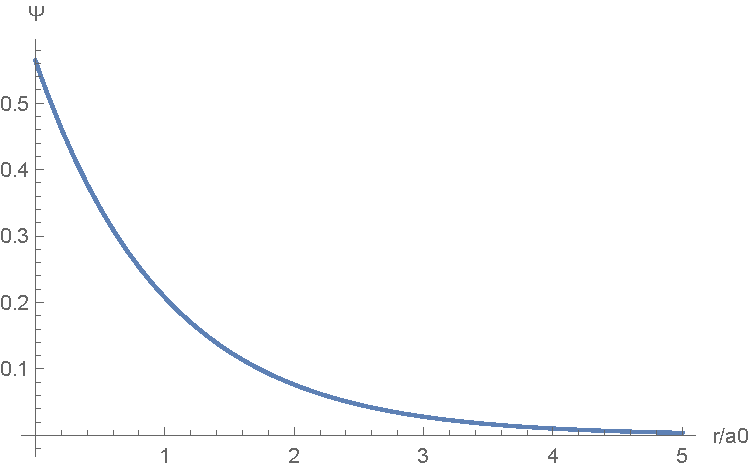
\includegraphics[width = 8cm]{itema.pdf}
\end{figure}

\subsubsection{b)mostre que P(r)dr=$|\psi(r)|^2 4 \pi r^2$dr; }
\subsubsection{c) Esboce P(r)x r e determine o raio em que é mais provável encontrar o elétron; }
\begin{figure}[H]
\centering
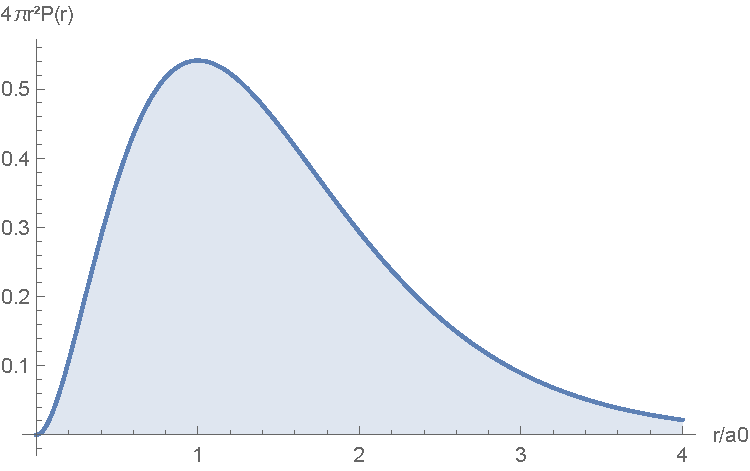
\includegraphics[width = 8cm]{item3c.pdf}
\end{figure}
\subsubsection{d)mostre que a função de onda dada é normalizada;}
\subsubsection{e)determine a probabilidade de encontrar o elétron na região $a_0/2<r<3a_0$/2.
}
\begin{figure}[H]
\centering
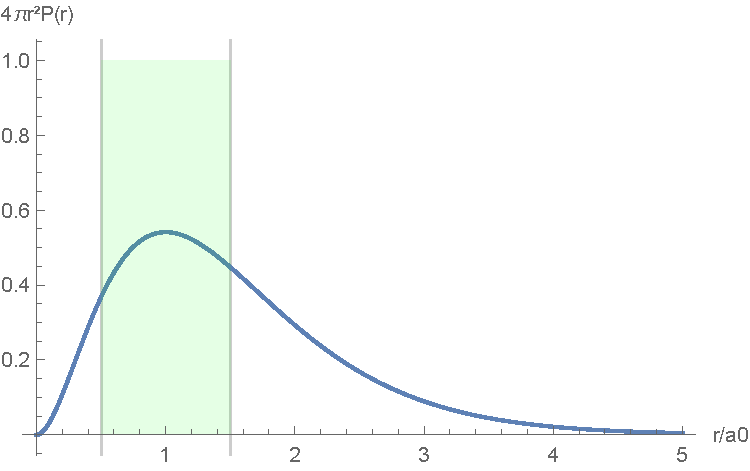
\includegraphics[width = 8cm]{item3e.pdf}
\end{figure}
Física Moderna 2 — Lista de exercícios 3

E and R, Cap. 11.
\section{Questões:}
\subsection{1 - O que descrevem exatamente os fatores de inibição e aumento? Qual é sua origem?}

O fator de inibição, presente na distribuição estatística de Fermions, reflete o princípio de exclusão de Pauli, já que implica que se uma particula se encontra em um estado, outra partícula não pode ficar no meu estado.
Já o fator de aumenta, da distribuição de bósons, demonstra que um bóson tende a ficar no estado em que se encontra outros bósons.


\subsection{3 - Qual a razão básica que explica ques as distribuições quânticas se confundem com a distribuição clássica para energias muito maiores do que kT?}
%386, 387
Quando a energia é muito maior que kT, a tendência é que o estado se encontre desocupado (ou seja, n $<<$ 1). O comportamento assintótico das três distribuições é o mesmo nesse limite.


\subsection{4 - Explique por que o comportamento da distribuição de Boltzmann se situa entre as distribuições de Bose e Fermi.}

Como 
\begin{equation}
    \frac{1}{e^{x}+1}<\frac{1}{e^{x}}<\frac{1}{e^{x}-1}
\end{equation}

para qualquer valor de x, então $n(E)_{Fermi} < n(E)_{Boltzmann} < n(E)_{Bose}$
para quaisquer valores de T.

\subsection{7 - Interprete fisicamente a energia de Fermi $\epsilon_F$}

\subsection{11 - Em nossa análise dos processos de emissão e absorção de um átomo num campo eletromagnético, desprezamos os efeitos de recuo. De que forma isso afeta nossos resultados? Fizemos bem em ignorar tais efeitos?}

\subsection{13 - Diz-se que um laser não é uma fonte de energia mas um conversor de energia. Explique.}
%396
A energia fornecida pelo laser não é mantida no átomo. Os elétrons de um átomo excitado por um laser voltarão ao mesmo nível de energia.

\subsection{17 - A baixas densidades e altas temperaturas, o gás de Bose se comporta como um gás ideal clássico. Explique esse resultado fisicamente.}
401, antes do exemplo

\subsection{21 - Nas equações do gás ideal usamos a massa de repouso das partículas. Por que nunca usamos a massa relativística? Considere o efeito da temperatura e a natureza da partícula.}
estamos supondo um gas classico, com v<<c

\subsection{23 - Na distribuição de Fermi deduzimos que na energia de Fermi $\epsilon_F$ o número médio de partículas por estado quântico é exatamente meio. Isso não é certamente o mesmo que dizer que 50 $\%$ das partículas está acima do nível de fermi e 50 $\%$ abaixo. Explique.}

386

\subsection{24 - Justifique a hipótese de que os elétrons de condução se comportam aproximadamente como um sistema de partículas livres que não interagem.}
%405
Isso é justificado porque, em um metal, os elétrons de condução tem mais mobilidade que os de valência e porque as forças de atração e repulsão vão, de forma aproximada, se cancelar.

\subsection{26 - Explique fisicamente o efeito de fazer h $\to$ 0 na expressão para a densidade de estados, como (11-49). Explique fisicamente o efeito de fazer h $\to$ 0 nas equações que envolvem o termo de degenerescência, como (11-53).}
%400,401
Na equação 11-49, o efeito é fazer com que o número de estados de um determinado intervalo de energia tenda a infinito.
Na equação 11-53, faz com que o termo de degenerescência tenda a zero e retomemos o resultado clássico.



\subsection{Por que um material, para poder ser usado como laser, deve ter pelo menos 3 níveis de energia?
}
O objetivo do laser é criar uma fonte de luz amplificada, ou seja, uma maior quantidade de fotos emitidos. Para isso, pela equação 11-41, é necessário que a proporção da população do estados mais energético pro menos energético seja maior que 1, mas tendência natural é oposta. Para isso, é necessário um mecanismo que mantenha a inversão de populações. Precisamos de um estado intermediário que seja metaestável, ou seja, que dure um tempo relativamente longo para que possa ser populado.

\pagebreak

\subsection{Considere um laser pulsado que usa um cristal de rubi como elemento ativo. O cristal (Al2O3) contém impurezas de Cr3+, que dão ao rubi sua cor vermelha. Suponha que essas impurezas configurem um sistema de 3 níveis cuja população é invertida e que a luz laser seja emitida em pulsos de 50 ns. O cristal de rubi contém 3x1019 íons de Cr3+. Se o comprimento de onda da luz emitida é 694,4 nm, determine:}
\subsubsection{a) a energia dos fótons em eV;}

\subsubsection{b) a energia total disponível em cada pulso, assumindo todos os íons Cr3+ no estado excitado;}

\subsubsection{c) a potência por pulso; }

\subsubsection{d) explique porque a potência obtida na prática é muito inferior à obtida em c).}


\subsection{Para um gás ideal em equilíbrio térmico, qual é a fração de moléculas cujas velocidades diferem em menos de 1 $\%$ da velocidade mais provável vp? Note que podemos aproximar $\Delta$v $\approx$ dv, neste caso.}

\subsection{Um sistema composto de N partículas idênticas tem distribuição de velocidades dada por  d$N_V$  = avdv, onde dNV é o número de partículas com velocidade entre v e v+dv, e a é uma constante. As velocidades variam entre 0 e V.
}
\subsubsection{Encontre a constante a em termos de N e V. 
}
\subsubsection{Calcule $v_m$ (velocidade média), $v_qm$ (velocidade quadrática média) e $v_p$ (velocidade mais provável) em termos de V.
}
\subsubsection{Calcule a porcentagem de partículas com velocidade entre $v_m$ e V.
}
\subsubsection{Calcule a porcentagem de partículas com velocidade entre $v_qm$ e V.
}
Física Moderna 2 — Lista de exercícios 3

E and R, Cap. 11.
\subsection{4 - Explique por que o comportamento da distribuição de Boltzmann se situa entre as distribuições de Bose e Fermi.}

Como 
\begin{equation}
    \frac{1}{e^{x}+1}<\frac{1}{e^{x}}<\frac{1}{e^{x}-1}
\end{equation}

para qualquer valor de x, então $n(E)_{Fermi} < n(E)_{Boltzmann} < n(E)_{Bose}$
para quaisquer valores de T.


\section{Problemas:}
\subsection{23 - Usando 197 como peso atômico e 9.7x10$^2$ kg/m$^3$ como densidade do ouro, calcule a profundidade do poço de potencial para elétrons livres no ouro. A função trabalho é 4.8 eV e existe um elétron livre por átomo.}
$E_F$ = 10.3 eV

\subsection{24 - Num sistema unidimensional, o número de estados de energia por unidade de energia é (l/h) $\sqrt{2m/\epsilon}$, onde l é o comprimento da amostra e m é a massa do elétron. Há $\mathcal{N}$ elétrons na amostra e cada estado pode ser ocupado por dois elétrons.}
%404
\subsubsection{a) Determine a energia de Fermi a 0k.}
$E_F = \frac{N^2\hbar^2}{32 m l^2}$


\subsubsection{b) Determine a energia média por elétron a 0k.}
$<E> = \frac{E_F}{3}$
\section{Outras}

\subsection{A energia de Fermi do cobre a 300 K é 7,05 eV. Determine:}
\subsubsection{a) a energia média de um elétron de condução do cobre;}
$<E> = \frac{3 E_F}{5}$ = 4.23 eV
(isso pode ser deduzido a partir da distribuição de Fermi)

\subsubsection{b) a temperatura na qual a energia média de uma molécula de gás ideal seria a mesma que a obtida em a).}
T = 32753 K


\subsection{A energia de Fermi do alumínio é 11,63 eV. Assumindo que o modelo de gás de elétrons livres seja aplicável ao alumínio, determine:}

\subsubsection{a) o número de elétrons livres por unidade de volume a temperaturas muito baixas;}
n = 1.82 x $10^{29}$ $m^{-3}$
\subsubsection{b) a valência do alumínio, dividindo a resposta de a) pelo número de átomos de Al por unidade de volume ($\rho_{Al}$ = 2,7 g/cm3 e $M_{Al}$ = 27 g).}
 = 1.82 x $10^{34}$ $m^{-3}$

\subsection{No Hg, a diferença de energia entre o primeiro estado excitado e o fundamental é 4,86 eV. Se uma amostra de Hg vaporizado em uma chama contém $10^{20}$ átomos em equilíbrio térmico a 1600 K, calcule:}

\subsubsection{a) o número de átomos nos estados n = 1 (fundamental) e n = 2 (primeiro excitado), usando o fator de Boltzmann e assumindo o mesmo peso estatístico para ambos;}

$n_1 \approx 10^{20}$
e $n_2 \approx 10^{4}$
\subsubsection{ b) a potência emitida pelos fótons emitidos na transição 2 $\to$ 1, se a meia-vida, $T_{1/2}$, do estado n = 2 é 100 ns. Lembre-se: Ptransição = $1/T_{1/2}$ e o número de fótons emitidos por unidade de tempo é $nP_{transicao}$.}

P =3.7 x $10^{-7}$ W
%392?


\subsection{Considere um laser pulsado que usa um cristal de rubi como elemento ativo. O cristal (Al2O3) contém impurezas de Cr3+, que dão ao rubi sua cor vermelha. Suponha que essas impurezas configurem um sistema de 3 níveis cuja população é invertida e que a luz laser seja emitida em pulsos de 50 ns. O cristal de rubi contém 3x1019 íons de Cr3+. Se o comprimento de onda da luz emitida é 694,4 nm, determine:}
\subsubsection{a) a energia dos fótons em eV;}

\subsubsection{b) a energia total disponível em cada pulso, assumindo todos os íons Cr3+ no estado excitado;}

\subsubsection{c) a potência por pulso; }

\subsubsection{d) explique porque a potência obtida na prática é muito inferior à obtida em c).}

(respondido na aula de revisão)


\subsection{Para um gás ideal em equilíbrio térmico, qual é a fração de moléculas cujas velocidades diferem em menos de 1 $\%$ da velocidade mais provável $v_p$? Note que podemos aproximar $\Delta$v $\approx$ dv, neste caso.}
Usar distribuição de Maxwell e encontrar $v_p$.

\begin{equation}
    N_{1\%} < \int^{(1.01)v_p}_{(0.99)v_p}
    4\pi \left(\frac{m_e}{2 \pi kT}\right)^{3/2}
    v^2e^{-m_0 v^2/2kT} dv
\end{equation}

\subsection{Um sistema composto de N partículas idênticas tem distribuição de velocidades dada por  d$N_V$  = avdv, onde $dN_V$ é o número de partículas com velocidade entre v e v+dv, e a é uma constante. As velocidades variam entre 0 e V.
}
\subsubsection{Encontre a constante a em termos de N e V. 
}
\subsubsection{Calcule $v_m$ (velocidade média), $v_{qm}$ (velocidade quadrática média) e $v_p$ (velocidade mais provável) em termos de V.
}
\subsubsection{Calcule a porcentagem de partículas com velocidade entre $v_m$ e V.
}
\subsubsection{Calcule a porcentagem de partículas com velocidade entre $v_{qm}$ e V.
}

(Respondido na aula de revisão.)

\subsection{1. A distância de equilíbrio entre os íons Rb+ e Cl- no RbCl é 0,279 nm.}

\subsubsection{(a) Calcule a energia  potencial de atração entre os íons, supondo que se comportem como cargas pontuais. }
\[V = \frac{-k e^2}{r} = -5.39 eV\] 

\subsubsection{ (b) A energia de ionização do rubídio é 4,18 eV e a afinidade eletrônica do cloro é 3,62  eV. Determine a energia de dissociação do RbCl, desprezando a energia de repulsão. }
\[E_{ion, tot} = E_{ion}-E_{afi} = 0.56 eV\]
\[E_{diss, teo} = -(V + E_{ion, tot}) = 4.38 eV\]
\subsubsection{(c) O valor experimental da energia de dissociação é 4,37 eV. Qual é a energia de repulsão  dos íons na distância de equilíbrio?}
%408 tipler 9-5
\[E_{diss, exp} = 4.37 eV = -(V+E_{ex} + E_{ion, tot} ),\]
onde $E_{ex}$ é a energia devido a repulsão. Então
\[E_{ex} = - 4.37 - 5.39 - 0.56 = 0.46 eV \]

(Para referência, ver exemplos 9.1 e 9.2, Tipler)

\subsection{2. A distância de equilíbrio da molécula de HF é 0,0917 nm e o valor experimental do  momento dipolar elétrico da molécula é 6,40 x $10^{-30}$ C m. Qual a porcentagem de  caráter iônico da ligação? }%9-12
Do enunciado,
\[d_{eq}= .097 \times 10^{-9} m\]
\[P_{exp}= 6.4 \times 10^{-30} C m\]

da teoria:

\[P_{teo}= q \times d_{eq} = 1.4672 \times 10^{-29} C m\]

então:

\[ion \% = P_{exp}/P_{teo} = 44\%\]

Para referência, exemplo 9.3, Tipler.

\subsection{3. A distância de equilíbrio da molécula de CsF é 0,2345 nm. Se a ligação é 70 $\%$ iônica, qual deve ser o valor do momento dipolar elétrico da molécula?} %9-13
Do enunciado,
\[d_{eq}= .02347 \times 10^{-9} m\]
\[ion \% = P_{exp}/P_{teo} = 70\%\]
Então:
\[P_{exp}= 0.7 P_{teo} = q \times d_{eq} = 2.62 \times  10^{-29} C m\]



\subsection{4. O momento dipolar p da molécula de água, representada de forma esquemática na Fig.  abaixo, é na verdade a soma vetorial de dois dipolos de módulos iguais, p1 e p2,  paralelos às retas que ligam o átomo de oxigênio aos dois átomos de hidrogênio. O  valor experimental do ângulo entre os dois átomos de hidrogênio é 104,5°, a distância  de equilíbrio entre o átomo de oxigênio e cada um dos átomos de hidrogênio é  0,0956 nm e o módulo de p é 6,46 x $10^{-30}$ C m. Determine a fração de carga que é  transferida de cada um dos átomos de hidrogênio para o átomo de oxigênio.} %9.16 tipler

\[p = p_1 \text{cos}(104.5/2) +p_2 \text{cos}(104.5/2)\]
    
Como os momentos de dipolo são iguais, vamos denominar
\[p_1=p_2 \equiv p_H\]

voltando,

\[p = 2p_H \text{cos}(52.25)\]
Assim,

\[p_H = \frac{p}{2\text{cos}(52.25)} = 5.27 \times 10^{-30} C m\]

\[p_{teo}  = q \times d = 1.53 \times 10^{-29} C m\]
Assim,

\[ion \% = P_{exp}/P_{teo} = 34\%\]

\subsection{5. A energia rotacional característica $E_{0 r}$ da molécula de N2 é 2,48 x $10^{-4}$ eV. A partir desta  informação, calcule a distância de equilíbrio dos átomos de nitrogênio na molécula de  N2.}  %9.20 tipler

\[E_{0 r} = \frac{\hbar}{2I}= \frac{\hbar}{2}\frac{2}{m_N r_0 ^2}\]

Usando \[E_{0 r} = 2.48 \times 10^{-4} eV= 3.97 \times 10^{-23} J\] e a massa do Nitrogênio,


\[r_0 = 1.098 \times 10^{-10}m\]
%%%%%%%%%%%%%%%%%%%%%%%%%%%%%%%%%%%%%%%%%%%%%%%%%%%%%%%%%%%%%%%%%%%%%
\pagebreak
\section{Extras}
\subsection{3- As resistividadese energias de Fermi do Na, do Au e do Sn, em T= 273 K, são 4,2 $\mu \Omega$.cm e 3,26 eV; 2,04 $\mu \Omega$ .cm e 5,55 eV; e 10,6 $\mu \Omega$ .cm e 10,3 eV, respectivamente. Use esses dados para determinar o caminho livre médio dos elétrons de condução desses materiais.}
%tipler 472 10-21
\[ \lambda_{Na} = 35.3 nm \]

\subsection{4- A energia total do gás de elétrons de condução em um metal, em função deT, pode ser aproximada por:
\[ U = \frac{3}{5}N E_F 
+ \alpha N \frac{k_T}{E_F} kT\],
com $\alpha \approx \pi ^2/4$
Use a expressão acima para deterrminar a energia média de um elétron no Cu em T=300 K. 
Compare esse resultado com a energia média em T = 0 K e com o resultado clássico, 3kT/2.}
% 10-23
\[ \langle  E \rangle_{300 K} =  4.24 \text{eV}\]
\[ \langle  E \rangle_{300 K, classico} = 0.038 \text{eV}\]

\subsection{5- Considere um pequeno cristal de Si, com 100 nm de aresta. a)Determineo número de átomos de Si, N, nesse cristal; b) Sabendo que a largura da banda de condução do Si tem 13 eV de largura e que existem 4N estados nessa banda, estime a diferença de energia entre estados adjacentes nessa banda.}
%10-30]
a) \[ N = 5 \times 10^7\]
b) \[ \Delta E = 6.5 \times 10^{-8} \text{eV}\]

\subsection{6- Uma fita de Sn tem 10 mm de largura e 0,2 mm de espessura. Um campo magnético B=0,25 T é aplicado perpendicularmente ao plano da fita, na qual passa uma corrente elétrica I= 20 A. Nesss condições, uma tensão Hall de 2,2 $\mu$ V émedida entre as laterais da fita. Sabendo que a massa atômica do Sn é 118,7 g/mole que sua densidade é r=5,8 g/cm3, determine: 
a) a concentração de portadores de carga; e 
b) o número de portadores por átomo de Sn.}
%10-35
a) \[ n = 7.1 \times 10^{28} m^{-3}\]
b) \[ n/N =  2.44 \text{elétrons por átomo}\]

\section{Eisberg and Resnick, Cap. 12}
 
\subsection{2. Você esperaria encontrar H3 num estado ligado? He2? Explique.}
%1298 serway
Não, já que haveria um átomo desemparelhado, o que não seria energeticamente favorável.

He2 também não, já que é um gás nobre (possui a última camada de valência ocupada, fazendo com que seja pouco reativo).

\subsection{6. Explique por que somente dois elétrons podem formar uma ligação covalente.}
%421, final
Porque os elétrons formam pares de spins diferentes. Tendo apenas duas possibilidades, só podem existir dois elétrons (antiparalelos) numa ligação covalente.

\subsection{8. Do fato de que o CO2 não tem um momento de dipolo elétrico permanente, o que se pode concluir sobre a ligação e a disposição dos átomos na molécula?}

Como essa molécula é composta por átomos diferentes, temos um momentode dipolo entre o Carbono e os Oxigênios. A configuração linear é a única em que possibilita que não haja momento de dipolo permanente, já que o momento de dipolo total é uma soma de seus componentes.

\subsection{9. Qual das três moléculas H2,D2 e HD tem a maior energia de ligação? Qual tem a menor?}
%429
Devido a energia de ponto zero, temos que, em ordem de maior para menor energia de ligação, $D_2$, HD, $H_2$.

\subsection{10. O que significa dizer que uma molécula se encontra num estado excitado?}
No contexto de molécula, pode significar tanto excitação rotacional, vibracional ou eletrônica.

\subsection{11. Explique por que a existência de uma energia vibracional do ponto zero finita está relacionada com o princípio de incerteza.}

O fato de que a energia vibracional de ponto zero seja finita condiz com a predição de um mínimo de energia de uma Hamiltoniana geral é maior que V0+(hbar omega)/2.

\subsection{12. A energia de vibração do estado fundamental do HCl é cerca de dez vezes maior do que a do NaCl. Mostre que isso é plausível considerando os fatores que determinam essa grandeza.}
%427
\[E_v = (\nu +1/2)h \nu_0\]

Do livro, temos que $h \nu_0$ = 0.04 eV para o NaCl enquanto, do exemplo, temos $h \nu_0$ = 0.37 eV para HCl. Faz sentido que a energia do NaCl seja menor, uma vez que é inversamente proporcional a massa reduzida da molécula, que é maior.

\subsection{14. Qual o efeito da mudança da separação internuclear devido a vibração (a curva de energia de ligação é assimétrica) sobre os níveis de energia rotacionais de uma molécula diatômica?}
%428, 430

A variação da mudança intermolecular vai alterar o momento de inercia, que é inversamente proporcional a energia rotacional.

\subsection{15.A assimetria na curva de energia de ligação explica a expansão térmica dos sólidos. Como se pode usar informação dos espectros moleculares para determinar a forma dessa curva?}

Pelo gráfico, é possível notar que espectros com energia de ligação mais profunda, ao receber energia térmica, terão menor alargamento da distância interatômica.

\subsection{16. Explique por que a separação entre os níveis vibracionais é ligeiramente menor num estado eletrônico excitado do que no estado eletrônico fundamental (veja figura 12-9). Explique o mesmo efeito para os estados rotacionais.}
%432, first parag?
Porque o aumento da energia torna a curva anarmônica e aproxima os níveis vibracionais. Os niveis rotacionais, sendo associados aos vibracionais, passam pelo mesmo.

\pagebreak

\section{Problemas}
\subsection{1. A distância de equilíbrio entre os íons Rb+ e Cl- no RbCl é 0,279 nm.}

\subsubsection{(a) Calcule a energia  potencial de atração entre os íons, supondo que se comportem como cargas pontuais. }
\[V = \frac{-k e^2}{r} = -5.39 eV\] 

\subsubsection{ (b) A energia de ionização do rubídio é 4,18 eV e a afinidade eletrônica do cloro é 3,62  eV. Determine a energia de dissociação do RbCl, desprezando a energia de repulsão. }
\[E_{ion, tot} = E_{ion}-E_{afi} = 0.56 eV\]
\[E_{diss, teo} = -(V + E_{ion, tot}) = 4.38 eV\]
\subsubsection{(c) O valor experimental da energia de dissociação é 4,37 eV. Qual é a energia de repulsão  dos íons na distância de equilíbrio?}
%408 tipler 9-5
\[E_{diss, exp} = 4.37 eV = -(V+E_{ex} + E_{ion, tot} ),\]
onde $E_{ex}$ é a energia devido a repulsão. Então
\[E_{ex} = - 4.37 - 5.39 - 0.56 = 0.46 eV \]

(Para referência, ver exemplos 9.1 e 9.2, Tipler)

\subsection{2. A distância de equilíbrio da molécula de HF é 0,0917 nm e o valor experimental do  momento dipolar elétrico da molécula é 6,40 x $10^{-30}$ C m. Qual a porcentagem de  caráter iônico da ligação? }%9-12
Do enunciado,
\[d_{eq}= .097 \times 10^{-9} m\]
\[P_{exp}= 6.4 \times 10^{-30} C m\]

da teoria:

\[P_{teo}= q \times d_{eq} = 1.4672 \times 10^{-29} C m\]

então:

\[ion \% = P_{exp}/P_{teo} = 44\%\]

Para referência, exemplo 9.3, Tipler.

\subsection{3. A distância de equilíbrio da molécula de CsF é 0,2345 nm. Se a ligação é 70 $\%$ iônica, qual deve ser o valor do momento dipolar elétrico da molécula?} %9-13
Do enunciado,
\[d_{eq}= .02347 \times 10^{-9} m\]
\[ion \% = P_{exp}/P_{teo} = 70\%\]
Então:
\[P_{exp}= 0.7 P_{teo} = q \times d_{eq} = 2.62 \times  10^{-29} C m\]



\subsection{4. O momento dipolar p da molécula de água, representada de forma esquemática na Fig.  abaixo, é na verdade a soma vetorial de dois dipolos de módulos iguais, p1 e p2,  paralelos às retas que ligam o átomo de oxigênio aos dois átomos de hidrogênio. O  valor experimental do ângulo entre os dois átomos de hidrogênio é 104,5°, a distância  de equilíbrio entre o átomo de oxigênio e cada um dos átomos de hidrogênio é  0,0956 nm e o módulo de p é 6,46 x $10^{-30}$ C m. Determine a fração de carga que é  transferida de cada um dos átomos de hidrogênio para o átomo de oxigênio.} %9.16 tipler

\[p = p_1 \text{cos}(104.5/2) +p_2 \text{cos}(104.5/2)\]
    
Como os momentos de dipolo são iguais, vamos denominar
\[p_1=p_2 \equiv p_H\]

voltando,

\[p = 2p_H \text{cos}(52.25)\]
Assim,

\[p_H = \frac{p}{2\text{cos}(52.25)} = 5.27 \times 10^{-30} C m\]

\[p_{teo}  = q \times d = 1.53 \times 10^{-29} C m\]
Assim,

\[ion \% = P_{exp}/P_{teo} = 34\%\]

\subsection{5. A energia rotacional característica $E_{0 r}$ da molécula de N2 é 2,48 x $10^{-4}$ eV. A partir desta  informação, calcule a distância de equilíbrio dos átomos de nitrogênio na molécula de  N2.}  %9.20 tipler

\[E_{0 r} = \frac{\hbar}{2I}= \frac{\hbar}{2}\frac{2}{m_N r_0 ^2}\]

Usando \[E_{0 r} = 2.48 \times 10^{-4} eV= 3.97 \times 10^{-23} J\] e a massa do Nitrogênio,


\[r_0 = 1.098 \times 10^{-10}m\]

\pagebreak

\section{Questões} 
%297 eisberg

\subsection{1. Explique a afirmação segundo a qual o princípio de exclusão impede que os sólidos  possam colapsar atingindo um volume nulo.}
%. 446 , serway 1296

The force between atoms is repulsive at very small separation distances. When two atoms are brought close to each other, some of their electron shells overlap, resulting in repulsion between the shells. This repulsion is partly electrostatic in origin and partly the result of the exclusion principle. Because all electrons must obey the exclusion principle, some electrons in the overlapping shells are forced into higher energy states and the system energy increases as if a repulsive force existed between the atoms

\subsection{2. Por que os sólidos metálicos são na maioria das vezes opacos, os sólidos covalentes  algumas vezes opacos e os sólidos iônicos raramente opacos à radiação visível? }
%. 444
A transparência ou não de um sólido depende da faixa de frequência necessária para excitar seus elétrons dentro do lattice. No caso ionico, essa frequência se encontra no UV, então a luz visível não é absorvida. A maior parte dos covalentes e metálicos, por sua vez, absorvem no visível.


\subsection{3. Entre as ligações: moleculares, iônicas, covalentes e metálicas, qual (ou quais) tem  maior chance de produzir um isolante? Um condutor? Um semicondutor? }
Condutor: metálica

Isolante: ionico (já que os ions estão restritos no lattice)

Semicondutor: Covalente

\subsection{4. Quais mecanismos explicam a resistividade elétrica comum dos metais? Quais dentre  eles dependem da temperatura? }
Flutuações térmicas e presença de impurezas. Impurezas não dependem da temperatura.
%.449,450

\subsection{5. Explique por que consideramos o preenchimento sequencial dos buracos por elétrons como equivalente a uma corrente positiva. Poderia este processo ser alternativamente  considerado como uma corrente de elétrons? }
%451

In some metals, as zinc and beryllium for example, the Hall effect indicates net positive charge carriers. This is interpreted as being due to transitions of electrons from the filled valence band to the conduction band leaving holes (unoccupied energy levels) in the valence band. 

Such holes correspond to the absence of an electron and behave much like positive charges. As these vacancies are filled by electrons, moving under the influence of an electric field, the holes move in a direction opposite to the electrons just as though positive charge carriers were moving in the field direction.

\subsection{6. Além de arsênico e antimônio, que outros elementos podem ser usados como  impurezas no germânio para formar um semicondutor de tipo n? Além do gálio e índio,  que outros elementos podem ser usados para formar um semicondutor de tipo p? }
Para tipo n, em geral, átomos com valência = 5.

Para tipo p, em geral, átomos com valência = 4.

%. 467-469

\subsection{7. A condutividade de um semicondutor pode ser afetada por bombardeio de elétrons?  Pelo bombardeio de outras partículas? }
O bombardeio de íons é uma técnica de dopagem (ion implantation).

\subsection{8. Qual o efeito de um campo elétrico aplicado num isolante? }
. pg 449
It is worthwhile putting the distinction between conductors and insulators into momentum, instead of energy, language. Without an applied electric field there are as many electrons in the solid with momentum vectors in one direction as there are with momentum vectors in the opposite direction, since there is no net current. When an electric field is applied, this equilibrium can be upset causing a current to flow, if some of the electrons can go into quantum states with changed momentum vectors. This is quite possible for electrons in a partially filled band, but it cannot be done by electrons in a completely filled band.

\subsection{9. Experimentalmente a adição de impurezas num metal aumenta sua resistividade  enquanto que a adição de impurezas num semicondutor diminui sua resistividade.  Explique. Entretanto, muitos isolantes não são muito puros. Por que as impurezas não  afetam a resistividade dos isolantes? }

Mesmo motivo da questão 8.

\pagebreak
\section{Problemas}

\subsection{1. Na figura abaixo, ilustramos de forma esquemática quatro distribuições de densidade  de carga de elétrons de valência em função da posição dos átomos, íons ou moléculas  (que aparecem como pontos na parte inferior da figura). Para cada distribuição (a), (b),  (c) e (d) qual tipo de ligação num sólido é mais condizente?}

%eisberg 298

a) Metálico (uniforme)

b) Iônico (ligação entre moléculas e evidentes intervalos alternados de cargas positivas e negativas)

c) Molecular (densidade mínima no meio da separação entre moléculas, indicando moléculas estáveis, que não estão em ligação covalente)

d) Covalente (como os eletrons são compartilhados, maior densidade de eletrons está no meio da separação das moléculas)



\subsection{2. Determine o tipo de ligação em cada um dos sólidos descritos abaixo. (a) O sólido  reflete a luz no visível; a resistividade elétrica aumenta com a temperatura; ponto de  fusão abaixo de 1000° C. (b) Reflete a luz no visível; a resistividade elétrica diminui  quando a temperatura aumenta; ponto de fusão acima de 1000° C. (c) Transmite a luz  no visível; só conduz eletricidade a temperaturas altas. (d) Transmite a luz no visível;  não conduz eletricidade em nenhuma temperatura. (e) Transmite a luz no visível; ponto  de fusão muito baixo.}

%eisberg 298
%serway 3 objective

a) Metálico

b) Covalente, não semicondutor

c) Covalente semicondutor

d) Ionico (conduz apenas quando derretido)

e) Molecular

\section{Extras}
\subsection{3- As resistividadese energias de Fermi do Na, do Au e do Sn, em T= 273 K, são 4,2 $\mu \Omega$.cm e 3,26 eV; 2,04 $\mu \Omega$ .cm e 5,55 eV; e 10,6 $\mu \Omega$ .cm e 10,3 eV, respectivamente. Use esses dados para determinar o caminho livre médio dos elétrons de condução desses materiais.}
%tipler 472 10-21
\[ \lambda_{Na} = 35.3 nm \]

\subsection{4- A energia total do gás de elétrons de condução em um metal, em função deT, pode ser aproximada por:
\[ U = \frac{3}{5}N E_F 
+ \alpha N \frac{k_T}{E_F} kT\],
com $\alpha \approx \pi ^2/4$
Use a expressão acima para deterrminar a energia média de um elétron no Cu em T=300 K. 
Compare esse resultado com a energia média em T = 0 K e com o resultado clássico, 3kT/2.}
% 10-23
\[ \langle  E \rangle_{300 K} =  4.24 \text{eV}\]
\[ \langle  E \rangle_{300 K, classico} = 0.038 \text{eV}\]

\subsection{5- Considere um pequeno cristal de Si, com 100 nm de aresta. a)Determineo número de átomos de Si, N, nesse cristal; b) Sabendo que a largura da banda de condução do Si tem 13 eV de largura e que existem 4N estados nessa banda, estime a diferença de energia entre estados adjacentes nessa banda.}
%10-30]
a) \[ N = 5 \times 10^7\]
b) \[ \Delta E = 6.5 \times 10^{-8} \text{eV}\]

\subsection{6- Uma fita de Sn tem 10 mm de largura e 0,2 mm de espessura. Um campo magnético B=0,25 T é aplicado perpendicularmente ao plano da fita, na qual passa uma corrente elétrica I= 20 A. Nesss condições, uma tensão Hall de 2,2 $\mu$ V émedida entre as laterais da fita. Sabendo que a massa atômica do Sn é 118,7 g/mole que sua densidade é r=5,8 g/cm3, determine: 
a) a concentração de portadores de carga; e 
b) o número de portadores por átomo de Sn.}
%10-35
a) \[ n = 7.1 \times 10^{28} m^{-3}\]
b) \[ n/N =  2.44 \text{elétrons por átomo}\]

\section{Questões}
\subsection*{1) Nas regiões do universo onde a energia térmica é kT $\approx 10^6$ eV, os processos atômicos são mais aparentes que os processos nucleares? E para as regiões onde kT $ \approx 10^{–6}$ eV?}
%eisberg q2. pg 550

Os processos atômicos possuem energias da ordem de eV, enquanto nucleares tem energias da ordem de MeV. Assim, regiões com kT $\approx 10^6$ eV, como no interior de estrelas, é ondem mais provavelmente teremos processos nucleares.

\subsection*{2) Todos os núcleos tem um momento monopolar elétrico (que mede sua carga total). Alguns núcleos tem um momento quadrupolar elétrico (que mede os desvios de suas distribuições de cargas em relação a uma simetria esférica). Nenhum núcleo tem um momento dipolar elétrico (que mediria a distância entre o centro de sua distribuição de carga e o centro de sua distribuição de massa). Por que não deveríamos esperar um momento dipolar elétrico para os núcleos?}
%q3
% https://physics.stackexchange.com/questions/273899/why-dont-the-nuclei-have-an-electric-dipole-moment
Por consideração de paridade - como a paridade do núcleo é bem definida, um operador ímpar como o momento de dipolo vai a zero.
%pg 518

\subsection*{3) Por que a unidade de massa não é definida em função da massa do átomo de hidrogênio? (Sugestão: Use a tabela 15-1 (E$\&$R) para fazer uma estimativa rápida da massa do ${}^{92}U^{238}$ considerando a massa do ${}^{1}H^{1}$ igual a 1.000000 u.)}
%q6
%pg 520 - 
Usa-se carbono pela abundância de hidrocarbonetos em ion sources.

%The singly ionized atomic mass can be determined from absolute measurements of the quantities on the right side of (15-9). But in practice use is made of various hydro-carbon molecules to calibrate the apparatus over a wide range of masses, in terms of the standard mass of carbon. The main reason that carbon is used as a standard, or unit, of mass is that many different hydrocarbons are readily available. In fact, the ion source usually produces some ionized hydrocarbons automatically, since hydro-carbons in the form of vacuum pump oil are present in the apparatus. The mass of the neutral atom can be obtained from that of the singly ionized atom by adding one electron mass. 

\subsection*{4) Uma vez que as seções atômicas e moleculares também envolvem energias de ligação, por  que  os  químicos  do  século  XIX  não  observaram  defeitos  de  massa  e  assim  não descobriram a teoria da relatividade?}
%q7

A defect mass que aparece na expressão relativística só é apreciável para energias grandes como as características de fenômenos nucleares.

\subsection*{5) Porque os núcleos mais estáveis se encontram na região próxima a A~60? Por que todos os núcleos não possuem A~60?}
%q9
%pg 525
É mais estável porque é a região onde E/A varia o mínimo possível. 
%Inspection of Figure 15-10 shows  that E/A actually maximizes at about 8.7 MeV for A $\approx$ 60.

Isso ocorreria de a energia por nucleon fosse proporcional ao número de nucleons. Isso não ocorre pois a força nuclear é de curto alcance. 
%If each nucleon in a nucleus exerted the same attraction on all the other nucleons, the binding energy per nucleon would continue to increase as more and more nu-cleons were added to the nucleus; that is, AE/A would be proportional to A. The extremely important fact that AE/A is not proportional to A is due, in part, to the short range of nuclear forces

\pagebreak

\section{Problemas}

\subsection*{1)}
\subsubsection*{a-Determine em MeV, a energia de atração gravitacional entre dois prótons esfericamente simétricos e cujos centros se encontram distantes de 2fm.}

\[E_{grav} = 5.8 \times 10^{-37} \text{MeV}\]

\subsubsection*{b-) Considerando essa mesma separação, repita os cálculos para a energia de repulsão coulombiana.}

\[E_{Coul} = 0.7 \text{MeV}\]

\subsubsection*{ c-) Compare os resultados precedentes com a energia de atração nuclear, que é aproximadamente -10 MeV para o sistema em questão.}
%p3

\[E_{Grav}/E_{Nuc} = 10^{-38}\]
\[E_{Coul}/E_{Nuc} = 0.01\]

\subsection*{2) Os núcleos ${}^5B^{11}$ e ${}^6C^{11}$ são chamados núcleos espelhos porque eles têm o mesmo número de núcleons, sendo que o número de prótons de um é igual ao número de nêutrons de outro. Se as forças nucleares não dependem da carga, as energias de ligação totais desses núcleos devem diferir apenas pela energia coulombiana, que é maior para ${}^6C^{11}$. A massa atômica do ${}^5B^{11}$ é 11,00930 u e a massa atômica do ${}^6C^{11}$ é 11,011432 u.}
% p16

\subsubsection*{a-Calcule a diferença entre suas energias de ligação totais.}

\[\Delta E_B = 76.32 MeV\]
\[\Delta E_C = 73.54 MeV\]
\[\Delta E_B - \Delta E_C = 2.78 MeV\]

\subsubsection*{b-Supondo que ambos os núcleos sejam esferas uniformemente carregadas e com o mesmo raior’, usea expressão de energia coulombiana (ver problema 11 do E $\&$ R) para encontrar o valor de r’ correspondente a uma diferença de energia coulombiana igual à diferença de energia de ligação.}

\[r' = 3.11 F\]

\subsubsection*{c-Compare este raio de distribuição de carga com a dependência radial da densidade de carga da figura 15.6 (E$\&$R).}
\[r_{figura}/r' \approx 0.8\]


\pagebreak

\subsection*{3) Use as massas que aparecem na tabela do Apêndice A (Tipler) para determinar a energia de ligação total e a energia de ligação por núcleon para os seguintes nuclídeos:}
%11.9
\subsubsection*{a - ${}^7Li$;}
B/A = 5.6 MeV/nucleon
\subsubsection*{b - ${}^{12}C$;}
B/A = 7.69 MeV/nucleon
\subsubsection*{c - ${}^{56}Fe$.}
B/A = 8.7 MeV/nucleon

\subsection*{4) Calcule a energia necessária para remover um nêutron:}
\subsubsection*{a-do ${}^{4}He$;}
E = 20.61 MeV
\subsubsection*{b-do ${}^{7}Li$;}
E = 7.26 MeV
\subsubsection*{c-do ${}^{14}N$.}
E = 10.6 MeV
%tipler 11.11, pg 554

\subsection*{5) Uma amostra de um isótopo radioativo tem uma atividade de 115,0 Bq no instante em que é retirada do reator nuclear responsável por sua formação. Depois de 2h 15 min, a atividade diminui para 85,2 Bq.}
%11.17

\subsubsection*{a-Calcule a constante de decaimento e a meia vida da amostra.}

\[\lambda = 0.133 h^{-1}\]
\[t_{1/2} = 5.2 h\]

\subsubsection*{b-Quantos núcleos radioativos havia na amostra?}
\[N_0 = R_0/\lambda = 3.11 \times 10^6\]

\pagebreak

\subsection*{6) O ${}^{80}Br$ pode sofrer os três tipos de decaimento $\beta$ .}
% A remains unchanged while Z and N change by +-1. These are $\beta-$ decay, in which a neutron insidea nucleus changes into a proton with the emission of an electron; $\beta+$ decay, in whicha proton inside a nucleus changes into a neutron with the emission of a positron; andelectron capture (EC), in which a proton in a nucleus changes to a neutron by captur-ing  an  atomic  electron, usually  a  1selectron  from  the  Kshell  since  these  have  thehighest probability density in the vicinity of the nucleus. Those nuclei on the neutron-rich side of the energy valley in Figure 11-15 will tend to decay by $\beta-$ emission, while those  on  the  proton-rich  side  will  most  probably  decay  by $\beta+$ emission  or  electron capture. We will discuss each of these processes briefly.

\subsubsection*{a-Escreva as equações de decaimento para os três casos.}

Os tres tipos de decaimento beta são $\beta-$, $\beta+$ e captura de elétron. Assim,

\[{}^{80}Br \to {}^{80}Kr + \beta^- + \bar{\nu}_e\]

\[{}^{80}Br \to {}^{80}Se + \beta^+ + \nu_e\]

\[{}^{80}Br \to {}^{80}Se + \nu_e \]


\subsubsection*{b-Calcule as energias de decaimento para os três casos.}
%11.34
\[E_{\beta_-} =  2 MeV\]
\[E_{\beta_+} =  0.85 MeV\]
\[E_{Captura de Eletron} =  1.9 MeV\]

\subsection*{7) O ${}^{3}He$ e o ${}^{3}H$ formam um par de nuclídeos especulares. Calcule a diferença entre as energias de ligação totais dos dois nuclídeos e compare o resultado com a energia de repulsão eletrostática dos prótons do ${}^{3}He$. Suponha que a distância entre os prótons é igual ao raio do núcleo de hélio.}
%11.78
\[\Delta E_{He} =  7.72 MeV\]
\[\Delta E_{H} =  8.5 MeV\]
Usar eq 11.5 para obter r e calcular repulsão:
\[\Delta E_{repulsao} = 0.83 MeV\]

\subsection*{8) Em um reator de fusão que utiliza apenas deutério como combustível, as reações mais frequentes são:
\[{}^{2}H + {}^{2}H \to {}^{3}He + n +3.27 MeV\]
e
\[{}^{2}H + {}^{2}H \to {}^{3}H + {}^{1}H +4.03 MeV\]
O ${}^{3}H$ produzido na segunda reação reage imediatamente com um núcleo de ${}^{2}H$:
\[{}^{3}H +{}^{2}H \to {}^{4}He + n + 17.7 MeV\]
A razão entre o número de átomos de ${}^{2}H$ e o número de átomos de ${}^{1}H$ no hidrogênio natural é 1,5x$10^{-4}$.
Qual será a energia produzida por 4 litros de água de todos os núcleos de ${}^{2}H$ sofrerem fusão?}
%11.88 tipler

A reação total é:

\[5 ({}^{2}H) \to {}^{1}H + {}^{3}He +{}^{4}He + 2n + 25 MeV\]

Energia por ${}^{2}H$ = 5 MeV.

4L de água = 444 $N_A$ átomos de hidrogênio, sendo a proporção de ${}^{2}H$ para ${}^{1}H$ é 1,5x$10^{-4}$.

Assim, energia para 4L de água = 2 $\times 10^{23}$ MeV = 32 GJ.

\section{Problemas}

\subsection*{7. A nucleossíntese primordial teve início quando o universo tinha ~1 ms e sua temperatura era ~$10^{10}$ K, de forma que prótons e nêutrons puderam se ligar formando dêuterons. Usando o fator de Boltzmann, as massas do próton (938,272 MeV/$c^2$) e do nêutron (939,566 MeV/$c^2$) e a temperatura, determine a razão do número de prótons para o de nêutrons: Np/Nn.}

\[ \frac{N_p}{N_n} = 4.5\]

\subsection*{8. O inverso do parâmetro de Hubble tem dimensão de tempo. Considere o valor de $H_0$=71 km/(s.Mpc). Lembrando que 1 pc = 3,26 anos-luz e que 1 ano tem ~ $\pi$ x $10^7$s, avalie a idade do universo considerando-a $H_0^{-1}$.}

\[t_{universo} \approx 4.33 \times 10^7 s\]

\subsection*{9. A energia gravitacional de uma esfera uniforme de massa M e raio R é:}
\[U_{grav} = \frac{-3 GM^2}{5 R}\]
\subsection*{A pressão de degenerescência de férmions (Pauli) é dada por: $P_{Pauli} = \frac{2 N \epsilon_F(0)}{3 V}$, sendo $\epsilon_F(0) = \frac{\hbar^2}{2 m} \left(\frac{3 \pi^2 N}{V}\right)^{2/3}$.}

\subsection*{Sabendo que as massas: $M_{\odot}$ ~ 2 x $10^{30}$ kg e do nêutron $m_n$= 1,675 x $10^{-27}$ kg, use esses dados para determinar o raio de uma estrela de nêutrons com M= $2M_{\odot}$.}

R = 4.48 km

\end{document}
